\chapter{Sample-level CNN using raw waveforms}
\textit{by Thorsten Wünsche}\\

In this chapter, we attempt to recreate an approach that reduces preprocessing by working with raw waveforms directly in a deep convolutional neural network. 

Section \ref{sec:theory} presents the original paper. In section \ref{sec:development}, we discuss the development process up until the first working prototype. Experiments and improvements to our own version are described in section \ref{sec:experiments}. Finally, section \ref{sec:conclusion} summarizes our experiences with this approach.

\section{Theory and original paper}
\label{sec:theory}
The paper "Sample-level Deep Convolutional Neural Networks for Music Auto-tagging Using Raw Waveforms" \cite{DBLP:journals/corr/LeePKN17} by Jongpil Lee, Jiyoung Park, Keunhyoung Luke Kim and Juhan Nam suggests an approach that works with raw waveforms directly. This differentiates it from our other models, which pre-compute entropy and MEL spectograms respectively.

Not only does this approach use raw waveforms, it also examines this data a few samples at a time, making it equivalent to pixel-level or character level when working with images and text respectively. 

Their suggested model consists of an initial convolution layer with equal filter length and stride, which combines a small number of samples into frames. These are then passed through $n$ convolution layer with filter length $m$ and stride one, each followed by a max-pooling layer with stride $m$. Each stage also makes use of batch-normalization and a ReLU activation function. Finally, the net ends with a fully connected layer with a $0.5$ dropout chance and a sigmoid output layer.

To allow for small values for both n and m (below 15), the input must be a short part of the song, between one and four seconds. The sample length of these tracks must be equal, as the dimensions of the model depend on it. The average of several segments is then used as the prediction.

After experimenting with different values for $m$ and $n$ as well as segment length, their most successful model uses $m=3$, $n=9$ and a segment length of 2678 ms at 22050 Hz. The structure of their model is shown in table \ref{tab:sample-dcnn_original-model}. For their learning rate, 0.01 is used as the initial value, reducing by a factor five after three consecutive epochs, in which the validation loss did not decrease. Training was halted while the learning rate was at 0.000016.

\begin{center}
	\begin{tabular}{ c c c c}
		
		layer & stride & output & \# of params\\
		\hline
		\hline
		conv 3-128 & 3 & 19683 x 128 & 512 \\
		\hline
		conv 3-128 & 1 & 19683 x 128 & 49280 \\
		maxpool 3 & 3 & 6561 x 128 & \\
		\hline
		conv 3-128 & 1 & 6561 x 128 & 49280 \\
		maxpool 3 & 3 & 2187 x 128 & \\
		\hline
		conv 3-256 & 1 & 2187 x 128 & 98560 \\
		maxpool 3 & 3 & 729 x 256 & \\
		\hline
		conv 3-256 & 1 & 729 x 256 & 196864 \\
		maxpool 3 & 3 & 243 x 256 & \\
		\hline
		conv 3-256 & 1 & 243 x 256 & 196864 \\
		maxpool 3 & 3 & 81 x 256 & \\
		\hline
		conv 3-256 & 1 & 81 x 256 & 196864 \\
		maxpool 3 & 3 & 27 x 256 & \\
		\hline
		conv 3-256 & 1 & 27 x 256 & 196864 \\
		maxpool 3 & 3 & 9 x 256 & \\
		\hline
		conv 3-256 & 1 & 9 x 256 & 196864 \\
		maxpool 3 & 3 & 3 x 256 & \\
		\hline
		conv 3-512 & 1 & 3 x 512 & 393728 \\
		maxpool 3 & 3 & 1 x 512 & \\
		\hline
		conv 1-512 & 1 & 1 x 512 & 262656 \\
		dropout 0.5 & - & 1 x 512 & \\
		\hline
		sigmoid & - & 50 & 25650 \\
		
		& & & \\	
	\end{tabular}
	\label{tab:sample-dcnn_original-model}
	\captionof{table}{The original model with the parameters Jongpil Lee, Jiyoung Park, Keunhyoung Luke Kim and Juhan Nam found to be the most successful. The layer "conv3-128 maxpool3" is to be understood as a one dimansional convolutio layer with filter length 3 producing 128 filters, followed by a maxpool layer with pooling length 3. The 50 in the sigmoid layer is the number of labels in the dataset (both MSD and MTAT, using the 50 most common tags).}
\end{center}


\section{Development and limitations}
\label{sec:development}

\begin{figure}[!htb]
	\centering
	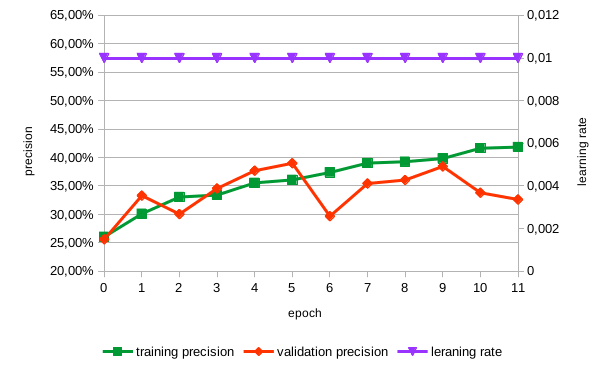
\includegraphics[width=.9\linewidth]{images/sample-dcnn-m3-n9-seg10-128_512-plateau.png}
	\caption{Performance of the $3^9$ model using 10 segments of music, between 128 and 512 filters and a reduce on plateau learning rate with the parameters suggested in the paper.}
	\label{fig:sample-dcnn-m3-n9-seg10-128_512-plateau}
\end{figure}


We created our own prototype by recreating the most successful model found by Jongpil Lee, Jiyoung Park, Keunhyoung Luke Kim and Juhan Nam. Their $3^9$ model shown in table \ref{tab:sample-dcnn_original-model} uses a one dimensional filter of size three in a convolutional neural network of depth 9 (1+9+1).  Using a frame-size of three, this model converts 59049 samples into 19683 frames. We also use the same sample rate (22050 Hz), so that each input into the model covers 2678 ms of audio.

The large FMA dataset \cite{fma_dataset} would not only take far too long to train on a desktop computer, but is also too large to be stored on the available hard drives. Therefore we use the small version of the dataset with 8000 songs (30 s each) distributed evenly across 8 top-level genres to adjust our model, before we attempt to classify the larger version on a server. Some of the files in the small dataset are corrupt or too short. Where not enough data for our model is available, the tensors are filled up with random numbers between - 1 and 1. As the defect files are in the single digits, this should not have a noticeable effect on the performance.

The performance of our initial implementation is shown in figure \ref{fig:sample-dcnn-m3-n9-seg10-128_512-plateau}. The learning rate scheduler does not seem to work as intended and possibly due to a constant learning rate of $0.01$, the accuracy leaves a lot to be desired. Even with these limitations, the model reaches an accuracy of 25\% on both the training and the validation set after a single epoch. In a balanced dataset with eight classes, this is already twice as good as a naive approach. The precision on both sets rises by 10-15 percentage points, though the validation precision declines soon after. All in all, this prototype works, but will need to be adapted to our hardware and time limitations.


\section{Experiments}
\label{sec:experiments}

Next, we will tweak the prototype described in section \ref{sec:development}. This will involve changing hyper-parameters as well as the filter-length and depth of the model. Using a CPU with eight virtual cores and a GeForce GTX 1060 6GB, the training of the prototype completed 12 epochs within eight hours. The following experiments are limited to this same timespan. This does mean that the model may not fully converge, but our primary concern is finding modifications that can increase the performance of our model before training it on the larger dataset using more capable hardware. 

\subsection{Learning rate}

\label{subsec:learning_rate}
\begin{figure}[!htb]
	\centering
	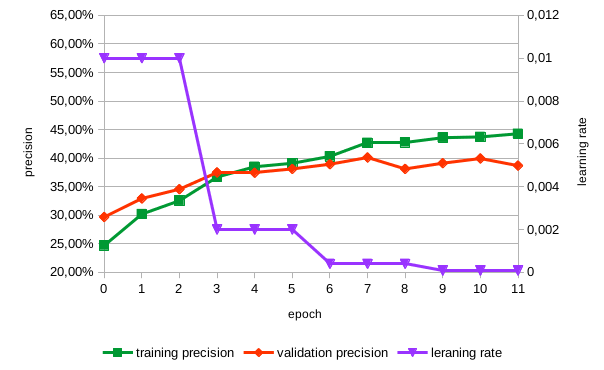
\includegraphics[width=.9\linewidth]{images/sample-dcnn-m3-n9-seg10-128_512-step.png}
	\caption{Performance of the $3^9$ model using 10 segments of music and between 128 and 512 filters. This version was modified to use a step learning rate dividing by a factor five every three epochs.}
	\label{fig:sample-dcnn-m3-n9-seg10-128_512-step}
\end{figure}

The first subject of experimentation is the learning rate. In the original prototype, we use the same model as Jongpil Lee, Jiyoung Park, Keunhyoung Luke Kim and Juhan Nam: The learning rate starts at $0.01$ and decreases by a factor five when the validation loss has not decreased in three consecutive epochs. In eight hours of training on a desktop computer, our prototype finished 12 epochs. This means that a quarter of the total training time would be required to identify a plateau. Indeed, during our initial training the learning rate was not reduced even once. With more time or faster hardware, this would be acceptable. We want to conduct a few other experiments as well however, and therefore tried two other approaches.

First, we keep the starting rate of $0.01$ and reduce it by the same factor five after three epochs regardless of the validation loss. This leads to three decreases over the course of one session. In the paper, training was halted after four decreases.

As can be seen in figure \ref{fig:sample-dcnn-m3-n9-seg10-128_512-step}, the accuracy on the validation set with our modification not only rises above 40\% at one point, it also remains much more stable, making it an overall improvement. The downside of this approach is, that after a few more epochs, the learning rate will be too low to allow for further improvement, even if the model and the dataset still had potential. As we plan to also apply our model to a larger dataset on more powerful hardware, this schedule might prove too limiting.

To adjust the learning rate in a more flexible manner, we return to the reduce on plateau scheduler, but make some adjustments to allow it to be effective even with limited time and hardware. We reduce the patience period from three to zero, reducing immediately upon a rise in the validation loss. As this makes the scheduler more vulnerable to small mistakes, we reduce the factor of the division from five to two and add a one epoch cooldown, to give the validation loss time to recover after the learning rate has been reduced.

The results are shown in figure \ref{fig:sample-dcnn-m3-n9-seg10-128_512-plateau_mod}. The validation accuracy is initially less stable, but ends up at similar values to the previous experiment, while the precision on the training set rises to above 50\%. Most importantly, this scheduler adapts itself to the dataset and slows down only when required, rather than at a constant and possibly too high speed.

We conclude, that our modified version of the reduce on plateau scheduler is an improvement on our limited hardware and will use this version in all experiments from here on out. On more powerful hardware however, the original version will likely be superior, as it is less susceptible to small fluctuations in the validation loss.


\begin{figure}[!htb]
	\centering
	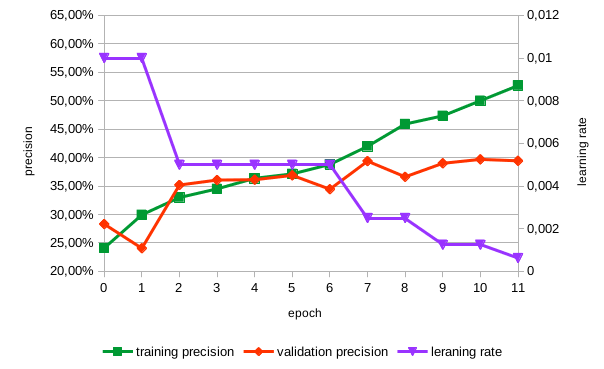
\includegraphics[width=.9\linewidth]{images/sample-dcnn-m3-n9-seg10-128_512-plateau_mod.png}
	\caption{Performance of the $3^9$ model using 10 segments of music and between 128 and 512 filters. This version was modified to use a reduce on plateau learning rate dividing by a factor 2 after every epoch, in which the validation loss did not fall. After every reduction, there is a one epoch cooldown to give the loss a chance to recover.}
	\label{fig:sample-dcnn-m3-n9-seg10-128_512-plateau_mod}
\end{figure}


\subsection{Number of filters}

In the paper, the authors experiment both on MTAT and MSD. For MTAT, increasing the number of filters in the convolution layers from 16 to 512 was sufficient, but performance on MDS improves when starting at 128 filters. Our prototype uses 128-512 filters initially, in this experiment, we reduce the number of filters in the earlier layers to 16 and gradually raise the number to 512. If this method results in a reduced training time without sacrificing accuracy, then the increased number of epochs may make up for the somewhat lower complexity.

\begin{figure}[!htb]
	\centering
	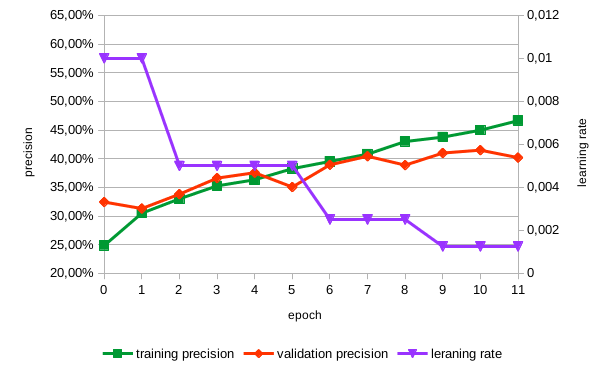
\includegraphics[width=.9\linewidth]{images/sample-dcnn-m3-n9-seg10-16_512-plateau_mod.png}
	\caption{Performance of the $3^9$ model using 10 segments of music and the modified reduce on plateau learning rate described in subsection \ref{subsec:learning_rate}. This version uses a reduced number of filters, increasing from 16 to 512 rather than 128 to 512.}
	\label{fig:sample-dcnn-m3-n9-seg10-16_512-plateau_mod}
\end{figure}

After training the model for eight hours, no significant decrease in training time was found. As shown in figure \ref{fig:sample-dcnn-m3-n9-seg10-16_512-plateau_mod}, the accuracy on the validation set however grew slightly, while the training precision fell significantly. This would suggest, that our previous model was overfitting to a small degree. Therefore we will keep using the reduced number of filters on the small dataset (8000 samples), but will increase it back to full for more complex applications.

\subsection{Number of segments}
\label{subsec:segments}

All models up to now have used ten segments of music, all of equal length, and averaged over the  results. We now reduce the amount of segments to one, hoping to achieve an increase in training speed without sacrificing too much accuracy.

\begin{figure}[!htb]
	\centering
	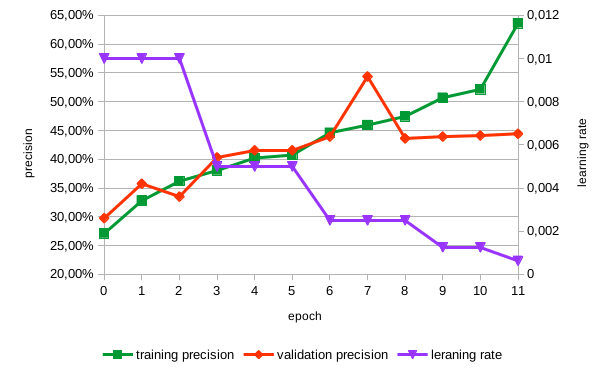
\includegraphics[width=.9\linewidth]{images/sample-dcnn-m3-n9-seg1-16_512-plateau_mod.png}
	\caption{Performance of the $3^9$ model using the modified reduce on plateau learning rate and a reduced number of filters, increasing from 16 to 512 rather than 128 to 512. This Version trains and classifies only one segment of music at a time.}
	\label{fig:sample-dcnn-m3-n9-seg1-16_512-plateau_mod}
\end{figure}

Figure \ref{fig:sample-dcnn-m3-n9-seg1-16_512-plateau_mod} shows, that this modification is very effective, reducing the time needed to train and evaluate one epoch on the small dataset from 43 minutes to only twelve. The reduced training time is most likely due to having the dataloader handle only three instead of 30 seconds of music. In our current system, the CPU is clearly the bottleneck and this change lightens the load, allowing the GPU to receive data quicker. Due to leaving the model training overnight, the total time spent is a bit longer than the initial eight hours. This allows for significantly more epochs, which in turn increases the validation accuracy by 5\% compared to all previous models. In the later epochs the training and validation accuracy are almost equal.

\begin{figure}[!htb]
	\centering
	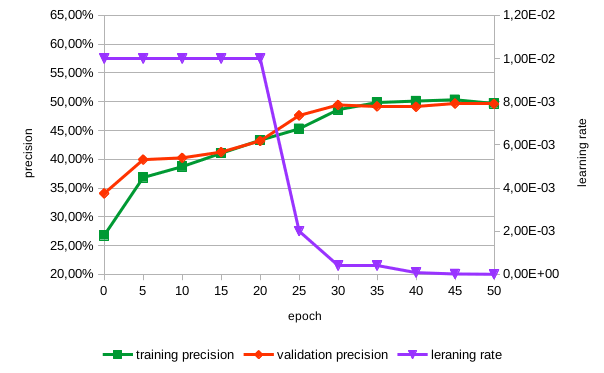
\includegraphics[width=.9\linewidth]{images/sample-dcnn-m3-n9-seg1-128_512-plateau.png}
	\caption{Performance of the first $3^9$ model using only one segment of music instead of ten.}
	\label{fig:sample-dcnn-m3-n9-seg1-128_512-plateau}
\end{figure}

The higher number of epochs also requires a reconsideration of the learning rate scheduler. In subsection \ref{subsec:learning_rate} we concluded that the original scheduler was too slow for our format. As the number of epochs can now realistically be quintupled, we return to the original settings, with only the number of segments reduced from ten to one. Figure \ref{fig:sample-dcnn-m3-n9-seg1-128_512-plateau} shows, that we were right to do so: Compared to the prevoius experiment, both training and validation accuracy increase by another 5\%, since the learning rate in the later epochs is not too small to prevent improvement. After epoch 46, the scheduler reduces the learning rate the fifth time, at which point Jongpil Lee, Jiyoung Park, Keunhyoung Luke Kim and Juhan Nam considered the training complete.

As the original model is now outperforms the other versions, we return to the full 128-512 filters and the reduce on plateau learning rate scheduler, which reduces after three epochs with no improvement to the validation loss.

\subsection{Depth and filter length}

We wanted to try changing the dimensions of the model in at least one experiment. Originally, a $3^6$ model was planned, hoping to reduce the training time. Now that subsection \ref{subsec:segments} has shown, that the CPU is our bottleneck, reducing the training time is no longer likely. We will instead train this model to find out how much of a difference the lower number of layers makes. If the depth can be reduced without lowering the accuracy significantly, this would make the model more suitable to being used on less powerful devices after the training is complete. 



\begin{figure}[!htb]
	\centering
	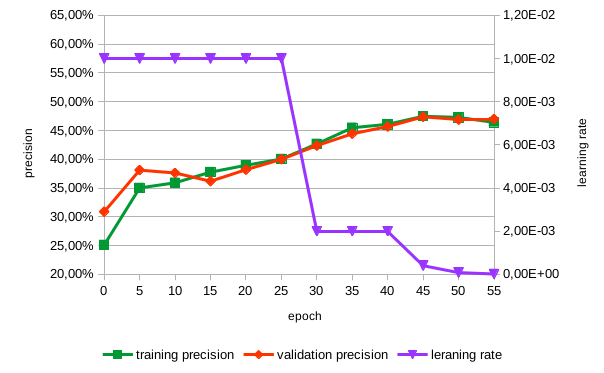
\includegraphics[width=.9\linewidth]{images/sample-dcnn-m3-n6-seg1-128_512-plateau.png}
	\caption{Performance of the $3^{6}$ model using one segment of music (2678 ms), the original reduce on plateau learning rate scheduler and 128-512 filters.}
	\label{fig:sample-dcnn-m3-n6-seg1-128_512-plateau}
\end{figure}

In figure \ref{fig:sample-dcnn-m3-n6-seg1-128_512-plateau}, we can see that the $3^{6}$ model reaches accuracy of about 3 percentage points under the $3^{9}$ version and requires more epochs to train. This may be very useful when applying the pre-trained model to weaker hardware, such as mobile devices, as the lower depth allows for faster classification. The lack of depth would likely cause significantly worse performance on more complex datasets.

To take advantage of the GPU power, which is currently going unused, we also train a deeper version. This new model uses 1+14+1 layers and a filter length and step size of 2. This model will not be able to use the same segments as our other versions, so we reduce the segment length to 32768 samples (1486 ms).

\begin{figure}[!htb]
	\centering
	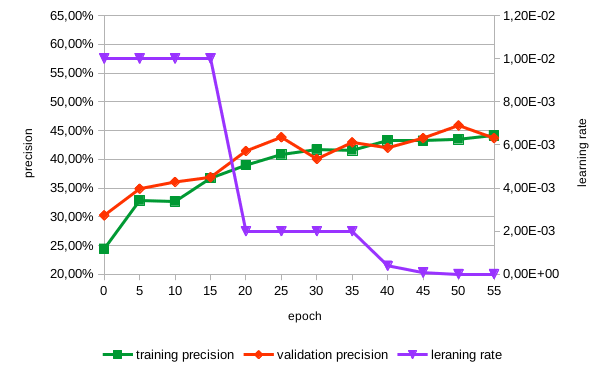
\includegraphics[width=.9\linewidth]{images/sample-dcnn-m2-n14-seg1-128_512-plateau.png}
	\caption{Performance of the $2^{14}$ model using one segment of music (1486 ms), the original reduce on plateau learning rate scheduler and 128-512 filters.}
	\label{fig:sample-dcnn-m2-n14-seg1-128_512-plateau}
\end{figure}

Figure \ref{fig:sample-dcnn-m2-n14-seg1-128_512-plateau} shows, that the  $2^{14}$ model requires more epochs to train than the  $3^{9}$ model, likely due to the added depth. The accuracy however is lower for both the training and validation set. This may be caused by the smaller filter, which requires a significantly higher number of layers to process longer inputs.

\section{Conclusion}
\label{sec:conclusion}

We were able to implement the model described in "Sample-level Deep Convolutional Neural Networks for Music Auto-tagging Using Raw Waveforms" \cite{DBLP:journals/corr/LeePKN17} and achieve a training and validation accuracy of 50\% on the small FMA dataset \cite{fma_dataset} within about ten hours on a desktop computer.

While we originally planned to train the best-performing model from the previous experiments on a server with the full dataset, this regrettably failed. The full set contains a number of files, that our dataset class was unable to load. These failures seemed to occur randomly, but frequently enough that training was not possible. As we found this problem fairly late in the project and both other team-members could use preprocessed data, thus bypassing this problem, we decided to use the remaining time to train the other two model using the more powerful hardware.

This approach is slow to train, since it requires large inputs, which have to be reloaded in each epoch. This puts a significant burden on the CPU, even if a powerful GPU is available.
Once the model is trained however, using it for predictions is fairly straight-forward. It can make reasonable predictions even with a small trainingset and using less than four seconds at a 22050 Hz sample rate. By making multiple predictions per song using different segments, misleading parts of a track can be overcome. Furthermore, by choosing segments at random during training, each song effectively can function as multiple different samples. The lack of pre-processing also makes this method suitable to being used on less powerful devices once the model has been trained.